\section{Future Work and discussion}

\subsection{Prototype heterogeneous cluster }
For the research of the difficulties and the feasibility of the operation of a software on different processor architectures a prototype is to be created and clod technologies are to use. Thus, for the construction of the infrastructure, a hererogenic Kubernetes cluster will be created, which contains both x86 and ARM processors. In the experiment itself it shall be shown that it is possible to run the same image of a program on both CPU architectures and to start containers created with the image alternately on both devices. 

\begin{figure}
	\centering
	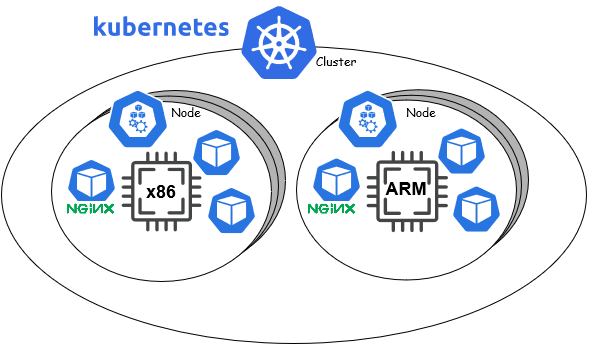
\includegraphics[width=.95\linewidth]{fig/experiment_k8s_cluster_x86_arm_v1.png}
	\caption{Prototype heterogeneous Kubernetes cluster.}
	\label{fig:prototypeKubeCluster}	
\end{figure}

The AWS Cloud will be used for the test setup. This offers users the choice of the two different processor types, including Arm and x86, which are to be used for the test. The image to be tested is nginx. This is already offered by the manufacturer in several versions for different CPU architectures, which eliminates the step of creating a separate test image. The web server nginx is also an excellent test example, since web servers are one of the most frequently used software on servers.

\subsection{Bench marking and calculating performance per watt on different workloads}
Since the first part of the test setup is to be implemented in the cloud of a provider for hardware and compatibility reasons, it is not possible to obtain data on the power consumption of the systems. Therefore, it was decided to set up a second series of tests with devices with the same CPU types, in which the computing power of devices is to be determined. While measuring the computing power by means of benchmarks, the energy consumption of the hardware is to be measured. The two values obtained can then be used to calculate the ratio of the computing power to the energy consumed in the process. the resulting ratios of the two architectures can then be used to compare the processor types with each other and make comparisons. The types of benchmarks performed can then be used to draw conclusions about which hardware can implement a more energy-efficient operation of a software.

\subsection{Bringing the experiments together}
The first experiment acts as a proof of concept of working heterogeneous CPU Clusters with current technology and to point out the limitations that occurred during the creation of the prototype. With the second Experiment measurable data was created that simulates a real life scenario. The used hardware used in this test represents hardware that might already be found  in a company. The created data during the experiment could later be used to create a power saving plan to decide what application should run on which hardware for the most power efficient use.
Creating a dedicated power saving plan and applying it to the created prototype of experiment one is not the goal of the following paper building up on this one. The goal of this paper and paper building up on it is limited to the demonstration of a working prototype of a cluster with heterogeneous CPU's and showing potential real world benefits of choosing the best suited CPU for a certain task.
